\documentclass[../../../main.tex]{subfiles}
\begin{document}
On s'est intéressé dans la première partie sur les graphes aux graphes non valués, c'est-à-dire pour lesquelles on n'associait pas de distances ni aucun autre genre de valeurs aux arcs.

On étend la définition d'un graphe orienté en ajoutant un valuation. On étend les représentations de même. On décrit de nouveaux algorithmes qui tiennent compte de cette valuation. On s'intéresse en particulier :
\begin{itemize}
	\item au calcul d'un arbre couvrant minimal d'un graphe
	\item au calcul du plus court chemin entre deux sommets d'un graphe
\end{itemize}
\subsection{Définition et représentations}
\definition{Graphe valué} {
	Un graphe valué sur $\mathbb{R}$ est un triplet $G = (S, A, c)$ où $c:A\rightarrow \ols{\mathbb{R}}$ est une fonction de valuation
qui à chaque arc associe une valeur. \newline
Si $(u, v)\notin A$, on a par convention $c((u, v)) = +\infty$\newline

Le poids d'un chemin $x_0\rightarrow \dots \rightarrow x_k$ est $c(x_0, x_1) + \dots + c(x_{k-1} , x_k)$.
}
\textbf{Valuations autres :} Le graphe pourrait être valué dans d'autres monoïdes que $(\mathbb{R}, +, 0)$. Le poids
n'a pas le même sens. Ci-dessous quelques exemples de monoïdes possibles :
\begin{itemize}
	\item $(\mathbb{N}, +, 0)$ ou $(\mathbb{R}, +, 0)$, le poids d'un chemin $\gamma = u\rightarrow^*v$ s'interprète comme le \textit{coût} de $\gamma$
	\item $([0, 1], \times, 1)$, un poids s'interprète comme une probabilité de changement d'état entre deux sommets
	\item $(\mathcal{P}(\Sigma^*), \dot, \{\varepsilon\})$\footnote{où $\Sigma$ est un alphabet, $\varepsilon$ est le mot vide, et où pour tous $A, B\in \mathcal{P}(\Sigma^*), A\dot B = \{ab\ |\ a\in A \wedge b\in B\}$}, le poids d'un chemin est langage, et un graphe valué est un automate\footnote{Automate généralisé, car d'ordinaire, le poids d'un arc est simplement un singleton $\{a\}\subset \Sigma^1$}.
\end{itemize}
\textbf{Exemple pour comprendre :} Le choix le plus commun de monoïde est $(\mathbb{N}, +, 0)$.\newline
Le graphe suivant est valué sur ce monoïde :
\begin{center}
	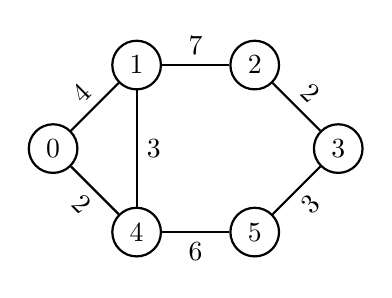
\begin{tikzpicture}[node distance={15mm}, thick, main/.style = {draw, circle}] 
	% Sommets :
	\node[main] (0) {$0$}; 
	\node[main] (1) [above right of=0] {$1$};
	\node[main] (2) [right of=1] {$2$};
	\node[main] (3) [below right of=2] {$3$};
	\node[main] (4) [below right of=0] {$4$};
	\node[main] (5) [right of=4] {$5$};
	% Arêtes
	\draw (2) -- node[midway, above, sloped] {7} (1);
	\draw (4) -- node[midway, right] {3} (1);
	\draw (4) -- node[midway, below, sloped] {2} (0);
	\draw (4) -- node[midway, below, sloped] {6} (5);
	\draw (2) -- node[midway, above, sloped] {2} (3);
	\draw (1) -- node[midway, above, sloped] {4} (0);
	\draw (3) -- node[midway, below, sloped] {3} (5);
	\end{tikzpicture} 
\end{center}
Le chemin $\gamma = 0\rightarrow 4 \rightarrow 1 \rightarrow 2 \rightarrow 3$ est de poids $2 + 3 + 7 + 2 = 14$. On peut donc dire que le coût du chemin $\gamma$ entre $0$ et $3$ est $14$.\newline
On observe que le plus court chemin entre $0$ et $3$ est $0\rightarrow 4 \rightarrow 5 \rightarrow 3$ (de poids $11$) selon la relation d'ordre usuel sur $\mathbb{N}$. On appelle le coût de ce plus court chemin la \textit{distance} entre $0$ et $3$.

Dans un graphe valué dans $\mathbb{N}$, on cherche généralement les chemins les plus courts, pour optimiser les
déplacements. Le calcul du chemin le plus court se fait généralement en calculant son coût.
\subsection{Signature du type abstrait}
On désigne par \textit{Monoide} le type abstrait associé au monoïde $(K, +, 0_K)$. Dans la pratique, \textit{Monoïde$\equiv$NombreRéel}

On étend la signature de graphe donnée dans la sous-section \ref{sub:signature_du_type_abstrait_graphe}. 

\textit{Graphe\textless Sommet, Monoide\textgreater} utilise \textit{Sommet}, \textit{Liste\textless Sommet\textgreater}, \textit{Entier}, \textit{Monoide} :
\begin{itemize}
	\item $poids(Graphe:G, Liste<Sommet>:l)\rightarrow Monoide$ renvoie le poids du chemin $l_1\rightarrow \dots \rightarrow l_n$ formé par les sommets de la liste $l$
\end{itemize}
\subsection{Représentations}
On enrichit ici les représentations de graphe données dans la sous-section \ref{sub:representations_graphe} en ajoutant la fonction de valuation du graphe évaluée sur chaque arc.
\subsubsection{Matrice par liste de successeurs}
On peut représenter un graphe valué $G = (S, A, V)$ par listes d'adjacence en enrichissant la structure de noeud de liste. On utilise une liste $Liste<Sommet, Poids>$ qui stocke à la fois les successeurs d'un sommet mais également le poids de l'arête. C'est-à-dire que pour tout $u\in S$, $succ(u) := \{(v, c(u, v))\ |\ u\rightarrow v\}$
\subsubsection{Matrice d'adjacence}
Dans le cas d'un graphe valué $G = (S, A, c)$ valué dans $\mathbb{R}$, la matrice d'adjacence $M\in\mathcal{M}_{|S|}(\mathbb{R})$ représentant $G$ est telle que :
$$\forall (u, v)\in S\times S, M_{u, v} = \left\{\begin{array}{ll}
c((u, v)) & \text{si } (u, v)\in A \\
+\infty & \text{sinon}
\end{array}\right.$$
\textbf{Remarque (l'infini en C) :} à partir de \textit{C99}, l'existence de la constante \textsf{INFINITY} de type \mintinline{c}{double}
est garantie par le standard dans le module \textit{math.h}, donc quelque soit le compilateur. Il faut penser à
ajouter le drapeau \textit{-lm} pour compiler.
\subsection{Premières propriétés}
\textbf{Notation :} Soit $G = (S, A, c)$ valué dans $\mathbb{R}$ et $x, y\in S$. On note $d(x, y)$ la borne inférieure des coûts
des chemins de $x$ à $y$ dans $G$.

\proposition{Distance} Soit $G = (S, A, c)$ un graphe valué dans $\mathbb{R}_+\setminus{\{0\}}$ non orienté. La
fonction $d : S^2\rightarrow \mathbb{R}_+$ telle que définie juste ci-dessus est une distance.

\textbf{Démonstration :} On vérifie les points suivants :
\begin{enumerate}
	\item symétrie ($\forall x, y\in S, d(x, y) = d(y, x)$) : OK puisque $G$ n'est pas orienté. Les chemins de $x$ à $y$
sont les mêmes que ceux de $y$ à $x$
	\item séparation ($\forall x, y\in S, d(x, y) = 0\Leftrightarrow x = y$) : OK car c est à valeur dans $\mathbb{R}_+\setminus\{0\}$
	\item inégalité triangulaire ($\forall x, y, z\in S, d(x, z)\leq d(x, y) + d(y, z)$) : OK par définition puisque $d$ est une
borne inférieure
\end{enumerate}
\textbf{Important :} Si la valuation est à valeur dans $\mathbb{R}$, on peut annuler le coût d'une arête par d'autres
arêtes de poids négatifs. Il est donc nécessaire pour avoir la séparation que la valuation soit à valeur
dans $\mathbb{R}_+\setminus\{0\}$

Le résultat suivant est assez facile, mais s'avère utile pour justifier plusieurs algorithmes par la suite.

\proposition{Sous-optimalité} Soit $G = (S, A, c)$ un graphe valué dans $\mathbb{R}$ et $x, y\in S$. Si
$\gamma : x = x_0\rightarrow \dots \rightarrow x_n = y$ est un chemin de $x$ à $y$ de coût minimal, alors pour tous $0\leq i \leq j \leq n$,
$x_i\rightarrow \dots \rightarrow x_j$ est un chemin de coût minimal entre $x_i$ et $x_j$.

\textbf{Démonstration :} Si un des sous-chemins n'était pas de coût minimal, on pourrait le remplacer par
un sous-chemin de coût minimal, formant ainsi un nouveau chemin $\gamma'$ de $x$ à $y$. $\gamma$ ne serait donc pas
de coût minimal, puisqu'on aurait $c(\gamma') < c(\gamma)$
\subsection{Algorithmes de Kruskal et Prim}
L'objectif des algorithmes de Kruskal et de Prim est de calculer l'arbre couvrant minimal d'un graphe
connexe non orienté.

La définition d'un arbre couvrant est donnée dans l'\refexercise{Arbres et graphes}.
\definition{Arbre couvrant minimal} {
	Soit $G = (S, A, c)$ un graphe connexe non orienté valué dans $\mathbb{R}$. Un arbre couvrant minimal est
un arbre couvrant de $G$ dont la somme des poids des arêtes est minimal\footnote{Parmi les sommes des poids des arêtes des autres arbres couvrants.}.
}
\subsubsection{Algorithme de Kruskal}
L'algorithme de Kruskal regarde le graphe ``de haut'' et choisit les plus petites arêtes au fur-et-à-mesure
pour coller les sommets. Il s'agit en fait de considérer chaque sommet une feuille. La liaison de deux
sommets va former un ``petit'' arbre. Lorsqu'on relie deux petits arbres, on a un plus ``gros'' arbre.
Lorsque toutes les feuilles sont reliés, on a un arbre couvrant.

On peut alors voir les sous-arbres comme une partition du graphe, et la liaison de deux sous-arbres
comme une union. Si deux sommets $x$ et $y$ sont dans le même ensemble de la partition, c'est qu'ils sont
déjà reliés dans un arbre. Il ne faut donc pas ajouter $(x, y)$ à l'arbre couvrant en construction, sinon on
crée un cycle.

On peut stocker chacune des arêtes du graphe dans une file de priorité, et simplement extraire de la
file les arêtes jusqu'à avoir un arbre.

\lemma{} Soit $G = (S, A, c)$. On note $T$ le graphe construit par l'algorithme de Kruskal sur $G$. Pour
tous $x, y\in S$, $x\rightarrow^* y$ dans $T$ est équivalent à $x\equiv y$ dans la partition.

\textbf{Démonstration :} On raisonne par récurrence sur la longueur $k$ des chemins entre $x$ et $y$ dans $T$. Pour
$k = 0$, on a $x = y$ donc $x\equiv y$. Soit un chemin $\gamma : x = x_0 \rightarrow \dots \rightarrow x_k = y$ dans $T$ de longueur $k > 0$.
Alors le chemin $x_0\rightarrow \dots \rightarrow x_{k-1} \neq 0$ est de longueur $k-1\geq 0$. Par HR, $x = x_0 \equiv x_{k-1}$. L'arête
$(x_{k-1} , y)$ a été ajouté en même temps que l'union de $x_{k-1}$ et $y$. Donc $x\equiv x_{k-1} \equiv y$.

\proposition{Correction de l'algorithme de Kruskal} L'algorithme de Kruskal termine et
est correct. Il calcule bien un arbre couvrant minimal de $G$.

\textbf{Démonstration :} La terminaison est immédiate de par la suppression itérée des éléments de la file.
Pour la correction, il faut vérifier deux points. D'abord que l'algorithme calcule effectivement un arbre
couvrant (c'est-à-dire connexe et acyclique), ensuite que cet arbre couvrant est minimal.
\begin{enumerate}
	\item Supposons que $T$ n'est pas connexe. Il existe donc au moins deux composantes connexes $T_1$ et $T_2$.
	Par connexité de $G$, il existe $x\in T_1$ et $y\in T_2$ tels que $(x, y)\in A$. Comme $x\not\rightarrow^* y$ dans $T$ , $x\not\equiv y$
d'après le lemme précédent. Or l'arête $(x, y)$ a été extraite à un $i^e$ tour de boucle quelconque de
la file de priorité. Si $x\not\equiv y$ au tour $i$, alors $x\equiv y$ au tour $(i+1)$. Ce qui est absurde puisque
$x\not\equiv y$ à la fin de l'exécution de l'algorithme. Donc $T$ est connexe, donc couvrant. \newline
Supposons qu'il existe un cycle dans $T$. Il existe donc un chemin $x\rightarrow^*y \rightarrow x$ dans $T$ (avec $x\neq y$). L'arête $(y, x)$ a été ajoutée à $T$ strictement avant ou strictement après la fermeture du
chemin $x\rightarrow^*y$. Dans le premier cas, la fermeture du chemin $x\rightarrow^*y$ n'est pas possible puisqu'on
a déjà $y\equiv x$. idem dans l'autre cas. \newline
Donc $T$ est connexe acyclique. Il est immédiatement couvrant puisque initialisé avec les sommets
de $T$.
	\item On procède par récurrence sur $0 \leq i \leq |S| - 1$ pour montrer que $T_i$ le graphe construit par
l'algorithme après le $i^e$ ajout d'arête est un graphe acyclique à $i$ arêtes minimales. Pour $i = 0$, c'est
le cas puisqu'il n'y a pas de coût possible. Supposons cette propriété vraie pour $0\leq i < |S| - 1$.
La $(i + 1)^e$ arête ajoutée est celle de coût le plus petit possible parmi celles hors de $T_i$ . En effet,
si une arête $(x, y)$ de coût encore plus petit avait été ajoutée, on aurait $x\equiv y$ avant l'ajout, donc
un cycle. Donc $T_{i+1}$ est minimal par HR. On a $T_n = T$ , donc $T$ est minimal.
\end{enumerate}
\begin{algorithm}
\caption{Algorithme de Kruskal\label{alg:kruskal}}
\KwIn{$Graphe:G = (S, A, c)$}
$Graphe:T = creer(|S|)$\tcp*{Arbre initialement vide}
$Partition:p = creer(|S|)$\;
$\textit{FilePriorite\textless Sommet, Sommet, Coût\textgreater}:file = creer\_vide()$\tcp*{La relation d'ordre de la file est sur le coût}
\ForAll {$x\in S$} {
	\ForAll {$y\in succ(G, x)$} {
		$inserer(file, (x, y, c(x, y)))$\;
	}
}
\While {$\neg est\_vide(file)$} {
	$Arc:(x, y)\leftarrow extraire\_minimum(file)$\tcp*{$log_2|A|$. $c(x, y)$ est ignoré car inutile autrement que pour l'ordre}
	\If {$trouver(p, x)\neq trouver(p, y)$} {
		$p\leftarrow unir(p, x, y)$\;
		$T\leftarrow ajouter\_arc(T, x, y)$\;
		$T\leftarrow ajouter\_arc(T, y, x)$\;
	}
}
\Return $T$\;
\end{algorithm}

On effectue $|S|$ opérations initialement pour construire l'arbre vide et la partition. Puis on fait $|A|$
tours de boucle pour chacune des opérations suivantes :
\begin{enumerate}
	\item insérer les arêtes dans la file de priorité (insertion de coût logarithmique)
	\item construction de l'arbre (extraction de la file de coût logarithmique)
\end{enumerate}
On note $C_{union}$ et $C_{trouver}$ les coûts des opérations $unir$ et $trouver$.

Le coût temporel de l'algorithme de Kruskal est donc fonction de $\Theta(|S|+|A|(log_2|A| + C_{union} + C_{trouver}))$.
Si on considère $C_{union}$ et $C_{trouver}$ en $\Theta(1)$, le coût temporel de l'algorithme de Kruskal est plus
simplement fonction de $\Theta(|S| + |A|log_2|A|)$.

\proposition{Unicité de l'arbre couvrant minimal} Si un graphe $G = (S, A, c)$ connexe non
orienté valué dans $\mathbb{R}$ est tel que pour tous $a_1 , a_2\in A$, $c(a_1)\neq c(a_2)$ (valuation des arêtes deux à deux
distincte sur $A$), alors il existe un unique arbre couvrant minimal de $G$.

\textbf{Démonstration :} Si il existe deux arbres $T_1$ et $T_2$ couvrant minimaux distincts d'un même graphe
$G$, alors il existe au moins une arête de $G$ avec $a\in T_1$ et $a\notin T_2$. On choisit celle de plus petit coût.
On peut alors ordonner les arêtes de $T_1$ selon leur coût par la liste $[a_1, \dots , a_{i-1} , u_i , u_{i+1} , \dots , u_{|S|-1} ]$ et
les arêtes de $T_2$ de même par la liste $[a_1 , \dots , a_{i-1} , v_i , v_{i+1} ,\dots, v_{|S|-1} ]$ où $i$ est le premier indice pour
lequel les deux suites diffèrent. On suppose sans perte de généralité que $c(u_i ) < c(v_i )$ On ajoute $u_i$ à
l'arbre $T_2$. Comme $T_2$ est acyclique maximal, $T_2\cup\{u_i\}$ possède un cycle. Comme $T_1$ est un arbre, ce
cycle n'est pas inclu dans $T_1$ . Donc il existe une arête $e$ de ce cycle qui n'appartient pas à $T_1$. $e$ est
donc une arête de $\{v_i ,\dots , v_{|S|-1}\}$. $T_3 = T_2 \cup \{u_i \} \setminus\{e\}$ est toujours connexe et a $|S| - 1$ arêtes donc
est un arbre couvrant. On a $c(T3 ) < c(T2 )$ car $c(ui ) < c(e)$ donc ni $T_1$ ni $T_2$ ne sont minimaux, ce qui
est absurde.
\subsubsection{Algorithme de Prim}
L'algorithme de Prim effectue un parcours du graphe qui garantit la minimalité de l'arbre de parcours
obtenu grâce à une file de priorité. L'algorithme de Prim voit donc le graphe ``de l'intérieur'', en se
promenant dedans, contrairement à l'algorithme de Kruskal qui le voit ``de haut''.

De fait, on peut préciser en entrée l'algorithme le point de départ $s_0$ du parcours. Comme le graphe
est connexe, on peut aussi choisir un sommet de départ arbitraire (comme $0$ si $S = \{1, \dots, n\}$).

La structure des algorithmes de Prim et Dijkstra et le parcours effectué par chacun des algorithmes
sont résolument identiques. La seule différence est que l'algorithme de Dijkstra effectue des calculs supplémentaires sur
des distances.

\begin{algorithm}
\caption{Algorithme de Prim\label{alg:prim}}
\KwIn{$Graphe:G = (S, A)$, $Sommet:s_0\in S$}
$\textit{Tableau\textless Booleen\textgreater }:sommets\_visites\left[|S|\right]$\;
\ForAll{$i\in S$}{
	$sommets\_visites[i] = \textit{Faux}$\;
}

$\textit{Graphe}:T = creer(|S|)$\;
$\textit{FilePriorite\textless Sommet, Coût\textgreater }:decouverts\leftarrow creer\_file\_vide()$\tcp*{La relation d'ordre de la file est sur le coût}
$decouverts \leftarrow enfiler(decouverts, (s_0, 0))$\;
\While {$\neg est\_vide(decouverts)$} {
	$Sommet:x\leftarrow defiler(decouverts)$\tcp*{$log_2|A|$. $c(x, y)$ est ignoré car inutile autrement que pour l'ordre}
	\If {$sommets\_visites[x] = \textit{Faux}$} {
		$sommets\_visites[x] = \textit{Vrai}$\;
		$T\leftarrow ajouter\_arc(T, x, y)$\;
		$T\leftarrow ajouter\_arc(T, y, x)$\;
		\ForAll {$y\in succ(G, x)$} {
			$decouverts\leftarrow enfiler(decouverts, (y, c(x, y)))$\;
		}
	}
}
\Return $T$\;
\end{algorithm}

\definition{Coupe} {
	Une coupe d'un graphe $G = (S, A, c)$ est une partition $C = \{S_1, S_2\}$ en deux sous-ensembles
des sommets de $G$, c'est-à-dire que $S = S_1 \sqcup S_2$ et $S_1\cap S_2 = \emptyset$.\newline
On note $A_C = (S_1\times S_2 )\cap A$ l'ensemble des arêtes de $G$ qui relient directement les sommets de
$S_1$ aux sommets de $S_2$.\newline

La coupe associée à un ensemble $S'\subset S$ est $C_{S'} = \{S', S\setminus S'\}$.
}
\definition{Sommets incidents} {
	Soit $G = (S, A)$ et $A' \subseteq A$. Les sommets incidents de $A'$ est l'ensemble des sommets :
$$\{u \in S\ |\ \exists v \in S/\{u, v\}\in A'\}$$
Pour tous $\{u, v\}\in A'$ , on a donc $u$ et $v$ des sommets incidents de $A'$
}

\proposition{Propriété fondamentale des arbres couvrants minimaux} Soit $G = (S, A, c)$.
Soit $T = (S, A_T)$ un arbre couvrant minimal de $G$ et $A'\subset A_T$. On considère la coupe $C = \{S', S \setminus S'\}$
associée aux sommets incidents de $A'$. On note $a\in A_C$ l’arête de coût minimal de $A_C$ . Alors il existe
un arbre couvrant minimal qui contient $A'\cup \{a\}$.

\textbf{Démonstration :} Si $a = \{x, y\}$ est une arête de $T$ , $T$ est un arbre qui convient. Sinon, comme $T$ est
un arbre couvrant, il existe une chaîne $x\rightarrow \dots \rightarrow y$ dans $T$. Il existe donc dans la chaîne une arête
$a' = \{x' , y'\}$ telle que $x'\in S'$ et $y'\in S \setminus S'$ . On pose alors $T' = T\cup\{a\} \setminus \{a'\}$. Comme $T'$ a $|S| - 1$
arêtes et est sans cycle (on a supprimé le seul cycle ajouté par $a$ en enlevant $a'$), alors $T'$ est un arbre
couvrant de G. Par ailleurs, $c(T') = c(T) + c(a) - c(a') \leq c(T)$ car $a$ est de coût minimal dans $A_C$.\newline
Donc $T'$ est un arbre couvrant minimal qui contient $A'\cup \{a\}$.

\proposition{Correction de l’algorithme de Prim} L’algorithme de Prim termine et est
correct. Il calcule bien un arbre couvrant minimal.

\textbf{Démonstration :} On visite chaque sommet du graphe une unique fois, donc l’algorithme effectue un
parcours. En particulier, il termine et construit bien un arbre couvrant. Pour la minimalité on montre
par récurrence sur $0 \leq i < |S| - 1$ que le graphe $T_i$ construit par l’algorithme de Prim après l’ajout de
la $i^e$ arête est toujours contenu dans un arbre couvrant minimal de $G$. En particulier, après l’ajout de
$|S| - 1$ arête, on a $T_{|S|-1}$ un arbre couvrant minimal.

\underline{Initalisation :} pour $i = 0$, aucune arête n’est ajouté. $G$ est non orienté connexe, donc il existe un arbre
couvrant minimal de $G$. Cet arbre contient $T_0$ qui est sans arêtes.

\underline{Hérédité :} Soit $0 \leq i < |S| - 1$. On considère les sommets déjà reliés par des arêtes dans $T_i$ (c’est-à-
dire les sommets incidents aux arêtes de $T_i$). Il s’agit des sommets déjà visités par l’algorithme. Les
sommets découverts sont exactement ceux accessibles depuis ces sommets. Cela forme une coupe $C$
entre les sommets visités et ceux non visités. $A_C$ est l’ensemble des arêtes qui vont de sommets visités
à des sommets non visités. L’algorithme de Prim ajoute $a\in A_C$ l’arête de coût minimal de $A_C$ pour
former $T_{i+1}$. D’après la \refproposition{Propriété fondamentale des arbres couvrants minimaux}, il existe un arbre couvrant minimal de $G$ qui contient $T_{i+1}$.
\subsection{Bellman-Ford}
On démontre les équations de Bellman pour justifier l'algorithme de Bellman-Ford, qui permet de
calculer en temps fonction de $O(|S|(|S| + |A|))$ la distance entre un sommet s et tous les autres
sommets du graphe. Cet algorithme peut être facilement adapté pour calculer le chemin de ce sommet
à tous les autres sommets par un tableau de prédécesseurs.

\textbf{Notation :} Soit $G = (S, A, c)$ valué dans $\mathbb{R}$. Pour tous $s, x\in S$, $k\in N$, on note $d_k(s, x)$ la borne
inférieure des coûts des chemins de $s$ à $s$ de longueur au plus $k$ dans $G$. Si aucun chemin de longueur
inférieure ou égale à $k$ n'existe, $d_k(s, x) = +\infty$.

$d_k(s, x)$ peut être compris comme une ``restriction'' de $d(s, x)$ aux chemins de longueur au plus $k$.

On commence par montrer par un premier lemme que $d_{|S|}(s, x)$ est ce qu'on veut calculer. On décrit
et démontre ensuite par un second lemme un moyen pratique de le calculer par récurrence sur $k$.

\lemma{} Soit $G = (S, A, c)$ un graphe valué dans $\mathbb{R}$ sans circuit de coût strictement négatif accessible
depuis $s\in S$, alors pour tout $x\in S$, $d(s, x) = d_{|S|}(s, x)$.

\textbf{Démonstration :} On a immédiatement $d(s, x)\leq d_{|S|}(s, x)$ puisque $d(s, x)$ est une borne inférieure. Comme $d_{|S|}(s, x)$ est optimal pour les chemins de longueur au plus $|S|$, on veut vérifier qu'il n'existe aucun chemin de longueur supérieure strictement
à $|S|$ qui soit plus court. Si un tel chemin $\gamma$ existe, par principe des tiroirs il existe forcément un
sommet $y\in S$ qui apparaît deux fois dans $\gamma$. Le chemin de $y$ à $y$ dans $\gamma$ est un cycle accessible depuis
$s$. D'après l'hypothèse, le coût de ce cycle est positif. L'enlever diminue le coût total de $\gamma$. Au final, on
peut enlever tous les doublons et avoir $|\gamma| \leq |S|$, donc $d(s, x)\geq d_{|S|}(s, x)$. On a double inégalité donc
égalité.

\lemma{Équations de Bellman} Soit $G = (S, A, c)$ un graphe valué sur $\mathbb{R}$. Pour tous $s, x\in S$ :
$$
\left\{
\begin{array}{llcl}
& d_0 (s, x) & = & \left\{\begin{array}{ll}
0 & \text{si }s = x \\
+\infty & \text{sinon}
\end{array}\right. \\

\forall k\in \mathbb{N}, & d_{k+1}(s, x) & = & min\left(d_k(s, x), min\{d_k(s, y) + c(y, x)\ |\ (y, x)\in A\}\right)
\end{array}
\right.
$$
\textbf{Démonstration : }
\begin{enumerate}
	\item Il y a un seul chemin de longueur 0 de $s$ à $s$. Il n'existe aucun autre chemin de longueur 0.
	\item Soit $k\in\mathbb{N}$. On a d'abord l'inégalité :
$$d_{k+1}(s, x)\leq min(d_k (s, x), min\{d_k(s, y) + c(y, x)\ |\ (y, x)\in A\})$$
puisque les chemins considérés dans le membre de droite sont tous de longueur au plus $(k+1)$.\newline
Soit $\gamma : s\rightarrow^* x$ de longueur $|\gamma|\leq k + 1$. Si $|\gamma|\leq k$, c'est terminé. Si $|\gamma| = k + 1 > 0$, on peut
écrire $\gamma = s\rightarrow^* y\rightarrow x$. Donc $d_{k+1} (s, x)\geq min\{d_k (s, y) + c(y, x)\ |\ (y, x)\in A\}$\newline
On a les deux inégalités, donc égalité.
\end{enumerate}

De cette récurrence on déduit un algorithme pour calculer les distances de $s$ à tout $x\in S$ par
mémoïsation des distances déjà calculés. C'est-à-dire qu'on garde en mémoire un tableau des distances
aux $|S|$ sommets qu'on maintient à jour au fur-et-à-mesure de l'algorithme pour ne pas avoir à le
recalculer. Le tableau final donne alors les distances de $s$ à tout $x\in S$ d'après le premier lemme.

\begin{algorithm}
\caption{Algorithme de Bellman-Ford\label{alg:bellmanford}}
\KwIn{$Graphe:G = (S, A, c)$, $Sommet:s$}
$Entier:n = |S|$\tcp*{Pour alléger l'écriture ensuite}
$Matrice:d\in \mathcal{M}_{S, \{0, n\}}(\mathbb{R})$\tcp*{\textsf{d[x][k]} donne $d_k(s, x)$}
\ForAll {$x\in S\setminus{\{s\}}$} {
	$d[x][0]\leftarrow +\infty$\;
}
$d[s][0]\leftarrow 0$\;
\For {$k\in [1, \dots, n]$} {
	\ForAll {$x\in S$} {
		$d[x][k] \leftarrow d[x][k-1]$\;
	}
	\ForAll {$x\in S$} {
		\ForAll {$y\in succ(G, x)$} {
			\If {$d[x][k-1] + c(x, y) < d[y][k]$} {
				$d[y][k] \leftarrow d[x][k-1] + c(x, y)$\tcp*{$x$ permet d'arriver à $y\Rightarrow x$ précède $y$ dans le parcours}
			}
		}
	}
}
\Return $d$\tcp*{Dernière ligne (la $(n+1)^e$) contient les distances de $s$ à $x$}
\end{algorithm}

D'après les deux lemmes précédents, l'algorithme est correct. L'algorithme effectue une boucle de
$n$ tours sur les valeurs de $k$. Pour chacun de ces tours, il parcourt tous les sommets puis tous les
successeurs de chaque sommet, c'est-à-dire toutes les arêtes. La complexité temporelle de l'algorithme
est donc fonction de $O(|S|(|S| + |A|))$ avec une représentation par listes d'adjacences si le calcul de
$c(x, y)$ est une opération élémentaire. Comme le coût d'une arête est stocké directement dans la liste
d'adjacence, c'est bon.

\textbf{Calcul des chemins :} L'algorithme ne donne pour l'instant que les distances. On peut obtenir les
chemins en eux-mêmes en ajoutant un tableau de prédécesseurs tel que $predecesseur[x] = y$ si l'arête
$(y, x)$ est une arête de l'arbre de parcours minimal, avec $predecesseur[s] = s$. La mise à jour a lieu à
la mise à jour de $d_k(s, x)$.
\subsubsection{Simplification de l'algorithme}
Il est en vérité possible d'appliquer l'algorithme de Bellman-Ford \textit{en place}. C'est-à-dire qu'au lieu d'avoir une matrice des $d_k(s, x)$ avec $k\in\{0, \dots, n\}$ et $x\in S$, on fait tous les calculs dans un seul tableau $d[x]$ qui prendra successivement les valeurs $d_0(s, x), \dots, d_n(s, x)$. En fin d'algorithme, on aura $d[x] = d_n(s, x)$ :

Que l'algorithme soit encore correct n'est pas évident au premier abord puisque les valeurs de $d$ semblent dépendantes à l'intérieur de la boucle. Toutefois la dépendance ne fait que diminuer les valeurs prises tout en restant des coûts de chemins réels nécessairement au dessus de la valeur minimale. Donc l'algorithme calcule toujours la valeur minimale.

\begin{algorithm}
\caption{Algorithme de Bellman-Ford simplifié\label{alg:bellmanfordsimplifie}}
\KwIn{$Graphe:G = (S, A, c)$, $Sommet:s$}
$Entier:n = |S|$\tcp*{Pour alléger l'écriture ensuite}
$\textit{Tableau\textless $\mathbb{R}$\textgreater}:d$\tcp*{\textsf{d[x]} donne $d_k(s, x)$ après le $k^e$ tour}
\ForAll {$x\in S\setminus{\{s\}}$} {
	$d[x]\leftarrow +\infty$\;
}
$d[s]\leftarrow 0$\;
\For {$k\in [1, \dots, n]$} {
	\ForAll {$x\in S$} {
		\ForAll {$y\in succ(G, x)$} {
			\If {$d[x] + c(x, y) < d[y]$} {
				$d[y] \leftarrow d[x] + c(x, y)$\tcp*{$x$ permet d'arriver à $y\Rightarrow x$ précède $y$ dans le parcours}
			}
		}
	}
}
\Return $d$\tcp*{Dernière ligne (la $(n+1)^e$) contient les distances de $s$ à $x$}
\end{algorithm}

\textbf{Démonstration (avec les mains) :} On montre que pour tout $k\in\{1, \dots, n\}$, on a $d[x] = d_{k}(s, x)$ après la boucle de la ligne $7$. On procède par récurrence. C'est vrai au début de l'algorithme, après l'initialisation des lignes 3 à 5. Supposons que cela soit vrai pour $k\in \{1, \dots, n-1\}$. Si $d[x]$ n'a pas été modifié depuis le début de la $k^e$ boucle, l'assignation à $d[y]$ est équivalente à celle de l'algorithme non simplifié. Sinon, comme $d[x] \leq d_k(s, x)$, $d[y]$ est inférieure ou égale à sa valeur dans l'algorithme non simplifié, c'est-à-dire $d[y] \leq d_{k+1}(s, y)$ à la fin du parcours des arêtes. Par ailleurs, la valeur correspond toujours au coût d'un chemin de longueur au plus $k+1$ vers $y$ donc $d[y]\geq d_{k+1}(s, y)$ puisque $d_{k+1}(s, y)$ est minimal. Donc pour tout $y\in S$, $d[y] = d_{k+1}(s, x)$.
\subsubsection{Détection des cycles à coût strictement négatif}
L'algorithme de Bellman-Ford peut être étendu pour détecter les cycles de coût strictement négatif accessibles depuis le sommet de départ. Dans le cas où de tels cycles existent, la distance entre le sommet de départ et un autre sommet est toujours $-\infty$ puisque le cycle peut être emprunté une infinité de fois.

Le lemme suivant permet de détecter les cycles à coût strictement négatifs :

\lemma{Cycles à coût strictement négatifs} Soit $G = (S, A, c)$ un graphe non orienté valué dans $\mathbb{R}$. Soit $s\in S$. Il existe un cycle de coût strictement négatif $z\rightarrow \dots \rightarrow z$ \textit{si et seulement si} il existe $y\in S$ tel que $d_{n+1}(s, y) < d_n(s, y)$.

Il suffit alors d'effectuer un tour de boucle supplémentaire dans l'\ref{alg:bellmanford} pour calculer $d_{n+1}$ et ajouter une boucle en fin d'algorithme pour vérifier que la condition de cycle négatif n'est pas vérifiée.

\textbf{Démonstration :}
\begin{enumerate}
	\item $(\Leftarrow)$ Si il existe $y\in S$ tel que $d_{n+1}(s, y) < d_{n}(s, y)$, alors il existe un chemin $\gamma:s\rightarrow^* y$ de longueur $(n+1)$ de $s$ à $y$ de coût strictement inférieur à tous les chemins de $s$ à $y$ de longueur au plus $n$. Par principe des tiroirs il existe un sommet qui se répète dans $\gamma$. Si le cycle déduit est de coût positif ou nul, on peut le supprimer et diminuer le coût de $\gamma$, qui est alors au plus de longueur $n$, ce qui n'est pas possible. Donc le cycle déduit est de coût strictement négatif.
	\item $(\Rightarrow)$ Puisqu'on peut supprimer les cycles des chemins de longueur $n+1$, on a toujours $d_{n+1}(s, y)\leq d_{n}(s, y)$. On a immédiatement $d_{n+1}(s, y) \geq d_n(s, y)$. Donc $d_{n+1}(s, y) = d_n(s, y)$. Par le même raisonnement, on a pour tout $k\in\mathbb{N}$ $d_{n+k}(s, y) = d_n(s, y)$. Supposons qu'il existe un cycle $z\rightarrow \dots \rightarrow z$ de longueur $k$ de coût strictement négatif accessible depuis $s$. On choisit $\gamma$ un chemin de longueur au plus $n$ qui relie $s$ à $z$. On peut concaténer à $\gamma$ le cycle strictement négatif. On a alors $d_{n+k}(s, z) < d_{n}(s, z)$, ce qui est absurde.
\end{enumerate}
\begin{algorithm}
\caption{Algorithme de Bellman-Ford avec détection des cycles négatifs\label{alg:bellmanford-detect}}
\KwIn{$Graphe:G = (S, A, c)$, $Sommet:s$}
$Entier:n = |S|$\tcp*{Pour alléger l'écriture ensuite}
$Matrice:d\in \mathcal{M}_{S, \{0, n\}}(\mathbb{R})$\tcp*{\textsf{d[x][k]} donne $d_k(s, x)$}
\ForAll {$x\in S\setminus{\{s\}}$} {
	$d[x][0]\leftarrow +\infty$\;
}
$d[s][0]\leftarrow 0$\;
\For {$k\in [1, \dots, n+1]$} {
	\ForAll {$x\in S$} {
		$d[x][k] \leftarrow d[x][k-1]$\;
	}
	\ForAll {$x\in S$} {
		\ForAll {$y\in succ(G, x)$} {
			\If {$d[x][k-1] + c(x, y) < d[y][k]$} {
				$d[y][k] \leftarrow d[x][k-1] + c(x, y)$\tcp*{$x$ permet d'arriver à $y\Rightarrow x$ précède $y$ dans le parcours}
			}
		}
	}
}
\ForAll {$y\in S$} {
	\If {$d[y][n+1] < d[y][n]$} {
		\Return Erreur : présence de cycle de coût strictement négatif\;
	}
}
\Return $d$\tcp*{Avant-dernière ligne ($(n+1)^e$) contient les distances de $s$ à $x$}
\end{algorithm}
\subsection{Algorithme de Dijkstra}
En restreignant encore les hypothèses et en supposant le graphe valué sur $\mathbb{R}_+\setminus\{0\}$ au lieu de $\mathbb{R}$, on
peut obtenir l'algorithme de Dijkstra de complexité temporelle fonction de $O(|E| + |S|log_2|S|)$. La
restriction est plus forte puisqu'au lieu d'interdire les circuits à coût strictement négatifs on interdit
les arcs à coût strictement négatifs.

\begin{algorithm}
\caption{Algorithme de Dijkstra\label{alg:dijkstra}}
\KwIn{$Graphe:G = (S, A, c)$, $Sommet:s_0\in S$}
$\textit{Tableau\textless{}Coût\textgreater}: d[|S|]$\tcp*{Tableau des distances}
$\textit{Tableau\textless{}Sommet \textgreater}: pred[|S|]$\tcp*{Tableau/arbre des prédécesseurs}
$\textit{Tableau\textless{}Booleen \textgreater}: sommets\_visites[|S|]$\;
\ForAll {$x\in S$} {
	$sommets\_visites[x] = \textit{Faux}$\;
	$d[x] = +\infty$\;
	$pred[x] = \texttt{Indéfini}$\tcp*{$-1$ par exemple}
}
$distance[s_0] = 0$\;
$\textit{FilePriorite\textless{}Sommet, Coût\textgreater}:file = creer\_vide()$ \tcp*{La relation d'ordre de la file est sur le coût}
$inserer(file, (s_0, 0))$\;
\While {$\exists s\in S/sommets\_visites[s] = \textit{Faux}$} {
	$Sommet:x = extraire\_minimum(file)$\tcp*{$d[x]$ est ignoré car inutile autrement que pour l'ordre}
	$sommets\_visites[x]\leftarrow \textit{Vrai}$\;
	\ForAll {$y\in succ(G, x)$} {
		\If {$d[y] > d[x] + c(x, y)$} {
			$d[y] \leftarrow d[x] + c(x, y)$\;
			$pred[y] \leftarrow x$\;
			\If {$\neg sommets\_visites[y]$} {
				$inserer(file, (y, d[y]))$\;
			}
		}
	}
}
\Return $d, pred$\;
\end{algorithm}

\subsection{Algorithme de Johnson}
L'algorithme ``classique'' pour calculer le plus court chemin entre chaque paire de sommets d'un graphe est l'algorithme de Floyd(-Warshall), qui est une généralisation de l'algorithme de Roy-Warshall. Cependant, cet algorithme est assez lent puisqu'il effectue le calcule en $O(|S|^3)$.

On montre ici l'algorithme de Johnson, qui effectue ces calculs en $O(|S||A| + |S|^2log_2|S|)$. Il construit un nouveau graphe à partir de $G$ sur lequel il applique d'abord Bellman-Ford puis itère l'algorithme de Dijkstra. 
\subsection{Exercices}
\end{document}